\chapter{Vector Architectures}
The basic principle underpinning a vector processor is the combination of two vectors to produce an output vector. If $A$, $B$ and $C$ are vectors of $N$ elements, a vector processor can perform the operation
\[ C = B + A \]
which is equivalent to
\[ C(i) = B(i) + A(i) \text{ where } 0 \le i \le N-1 \]

\begin{figure}
\centering
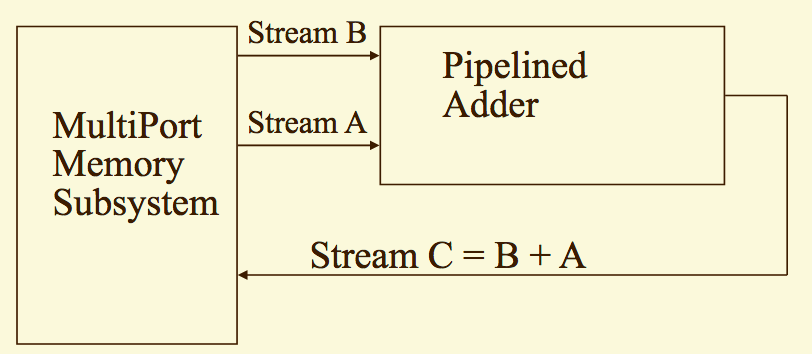
\includegraphics[width=0.7\linewidth]{figures/screenshot072}
\caption{Memory system for a vector processor.}
\label{fig:screenshot072}
\end{figure}

The memory subsystem for a vector processor needs to be able to support 2 reads per cycle and 1 write per cycle. This is illustrated in \autoref{fig:screenshot072}.

A vector processor is interesting as it can be used to dramatically speed up computation for operations over vectors. Consider unvectorised computation in \autoref{fig:screenshot073}, and vectorised computation in \autoref{fig:screenshot074}. The former is naive and must reload all state at the start of each computation; as a result, it must spend $N(t_1 + t_2 + t_3)$ time (where $t_1$, $t_2$ and $t_3$ are the pre-computation, computation, and post-computation times respectively) to evaluate $N$ results. The latter can compute multiple results simultaneously, allowing it to reduce the time to process $N$ elements to $t_1 + Nt_2 + t_3$ (i.e. setup, computation for $N$ elements, followed by teardown).

\begin{figure}
\centering
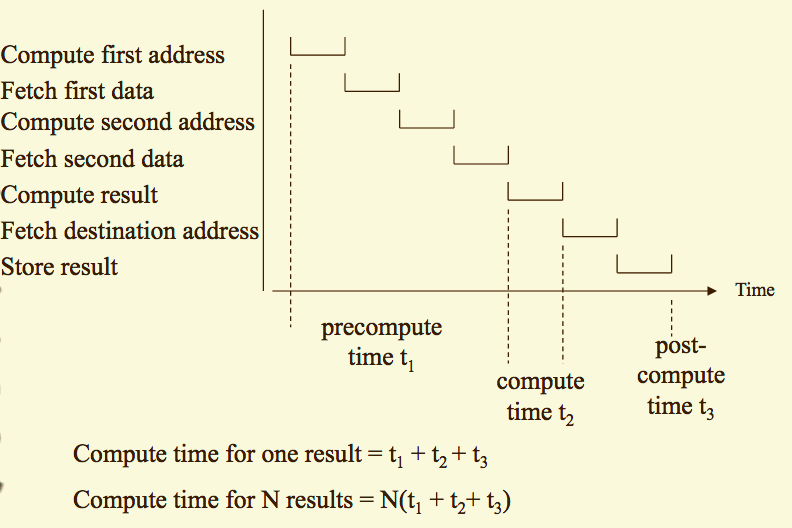
\includegraphics[width=0.7\linewidth]{figures/screenshot073}
\caption{Unvectorised computation.}
\label{fig:screenshot073}
\end{figure}

\begin{figure}
\centering
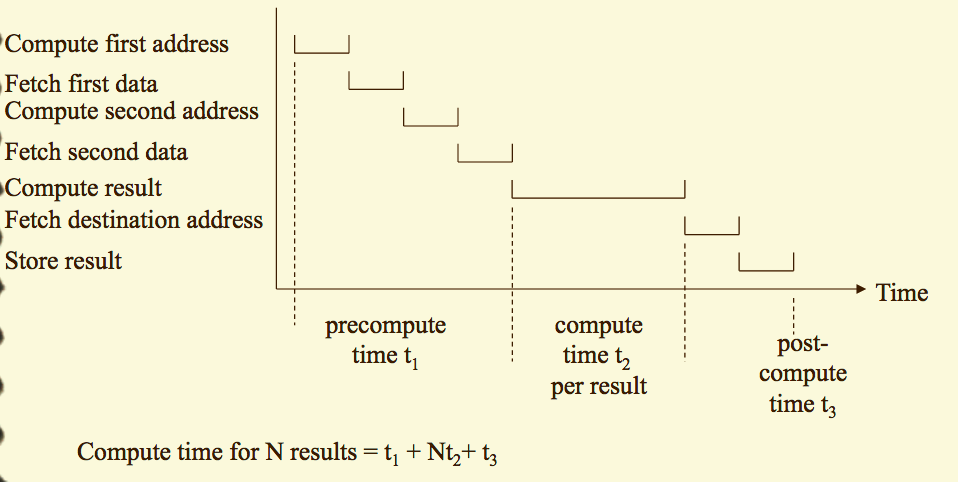
\includegraphics[width=0.7\linewidth]{figures/screenshot074}
\caption{Vectorised computation.}
\label{fig:screenshot074}
\end{figure}

This is made possible through the existence of pipelining, discussed in \autoref{chap:ilp}. This is shown in \autoref{fig:screenshot075} and \autoref{fig:screenshot076}, which showcase non-pipelined (i.e. serial) and pipelined (i.e. vectorised) computation respectively. Note that the execution time of a pipeline will always be bounded by its slowest component; this can be improved by increasing the granularity of the pipeline by increasing the number of stages. However, increasing granularity has its drawbacks, especially with regards to dependencies (discussed in \autoref{sec:dependencies}).

\begin{figure}
\centering
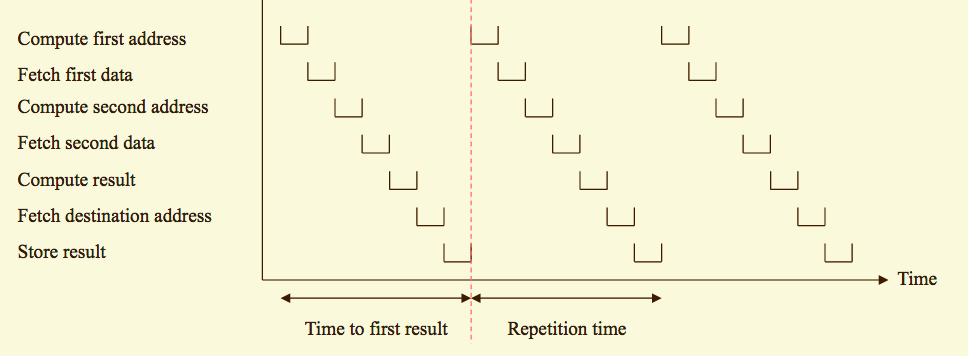
\includegraphics[width=0.7\linewidth]{figures/screenshot075}
\caption{Non-pipelined computation.}
\label{fig:screenshot075}
\end{figure}

\begin{figure}
\centering
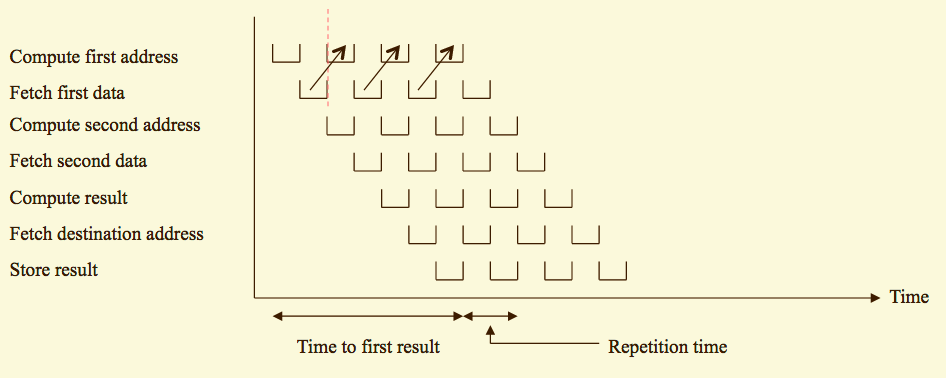
\includegraphics[width=0.7\linewidth]{figures/screenshot076}
\caption{Pipelined computation.}
\label{fig:screenshot076}
\end{figure}

\section{Interleaving}
For vector pipelining to work, it must be possible to fetch instructions from memory quickly. This is typically achieved through the use of cache memories (which caches repeatedly-accessed and upcoming instructions in CPU-local memory for rapid access), and interleaving (which will be discussed).

Conventional memory, seen in \autoref{fig:screenshot077}, consists of a set of storage locations accessed with some sort of address decoder. However, this means that there can be only one execution unit accessing the memory at any given time, preventing access from other EUs.

\begin{figure}
\centering
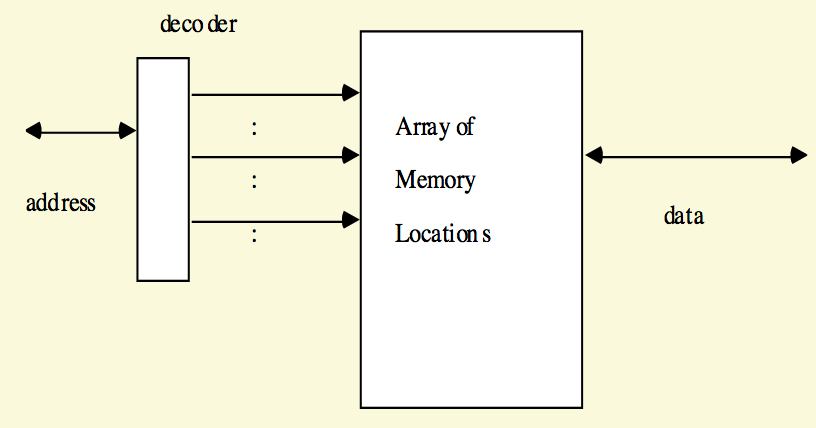
\includegraphics[width=0.5\linewidth]{figures/screenshot077}
\caption{Conventional memory.}
\label{fig:screenshot077}
\end{figure}

An interleaved memory system, seen in \autoref{fig:screenshot078}, uses a number of banks which correspond to a certain range of addresses. This effectively partitions the memory into multiple sections which can be concurrently accessed. Banks are usually selected using some of the low-order bits of the address (i.e. the least-significant bits) to ensure that sequential access will access different banks.

\begin{figure}
\centering
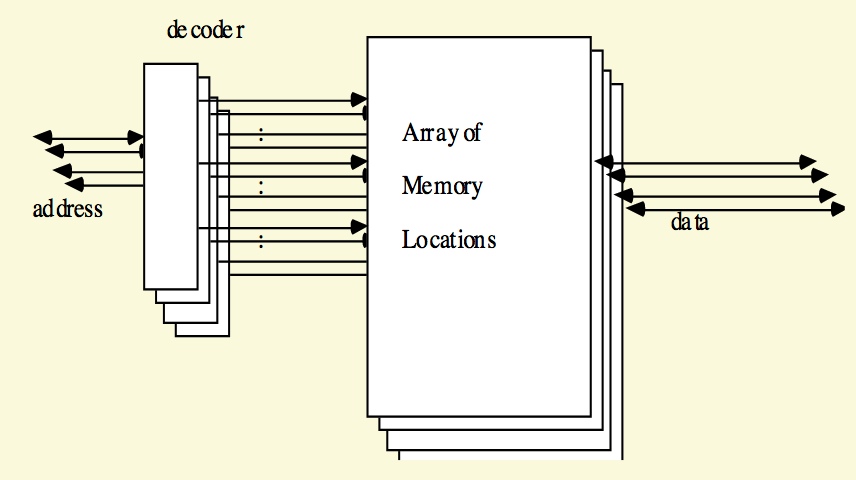
\includegraphics[width=0.7\linewidth]{figures/screenshot078}
\caption{Interleaved memory.}
\label{fig:screenshot078}
\end{figure}

A pipelined machine can be kept fed with instructions even though the main memory may be quite slow. An interleaved memory system slows down when subsequent accesses are for the same bank of memory. However, this is rare when prefetching instructions, because they tend to be sequential; as mentioned previously, banks are chosen to minimise the impact of sequential access. Additionally, it is possible to access two locations at the same time if they reside in different banks.  

\begin{figure}
\centering
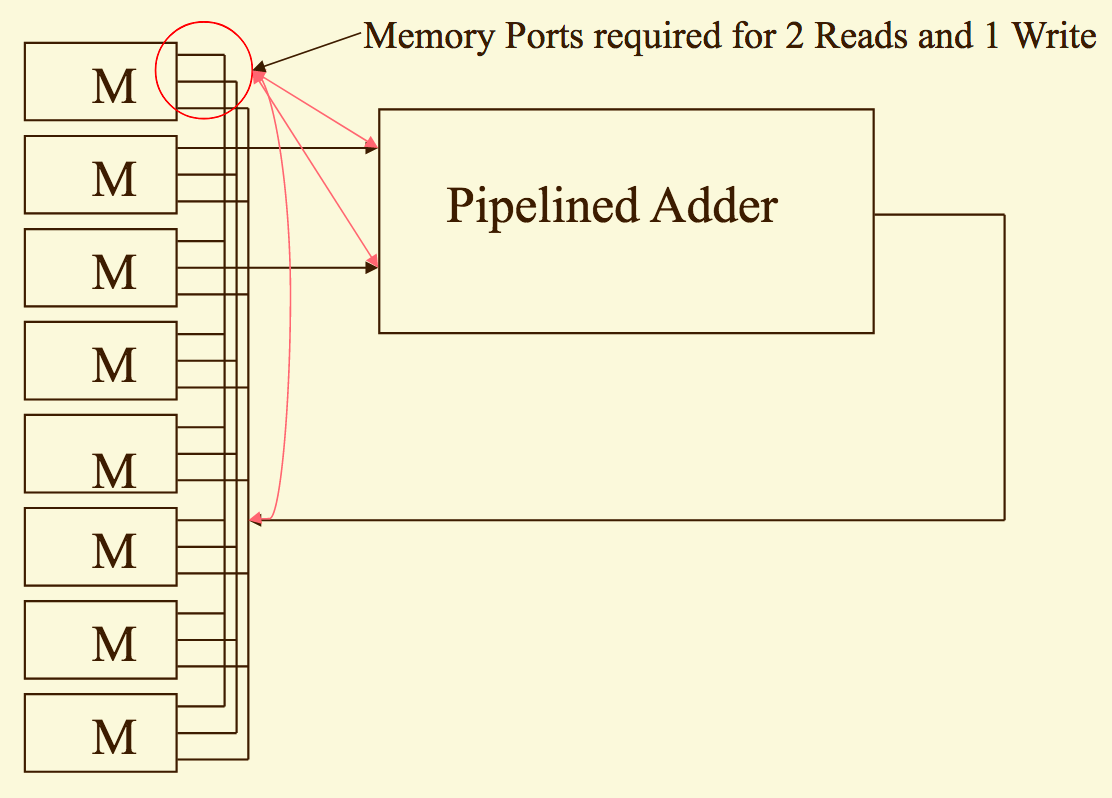
\includegraphics[width=0.7\linewidth]{figures/screenshot079}
\caption{Pipelined adder fed by an interleaved memory system.}
\label{fig:screenshot079}
\end{figure}

The use of multiple banks can be seen in context in \autoref{fig:screenshot079}, which uses two memory banks for its input and one memory bank for its output. This is further detailed in \autoref{fig:screenshot080} and \autoref{fig:screenshot081}, which depict the memory layout used for the adder and the utilisation of CPU pipelines respectively.

\begin{figure}
\centering
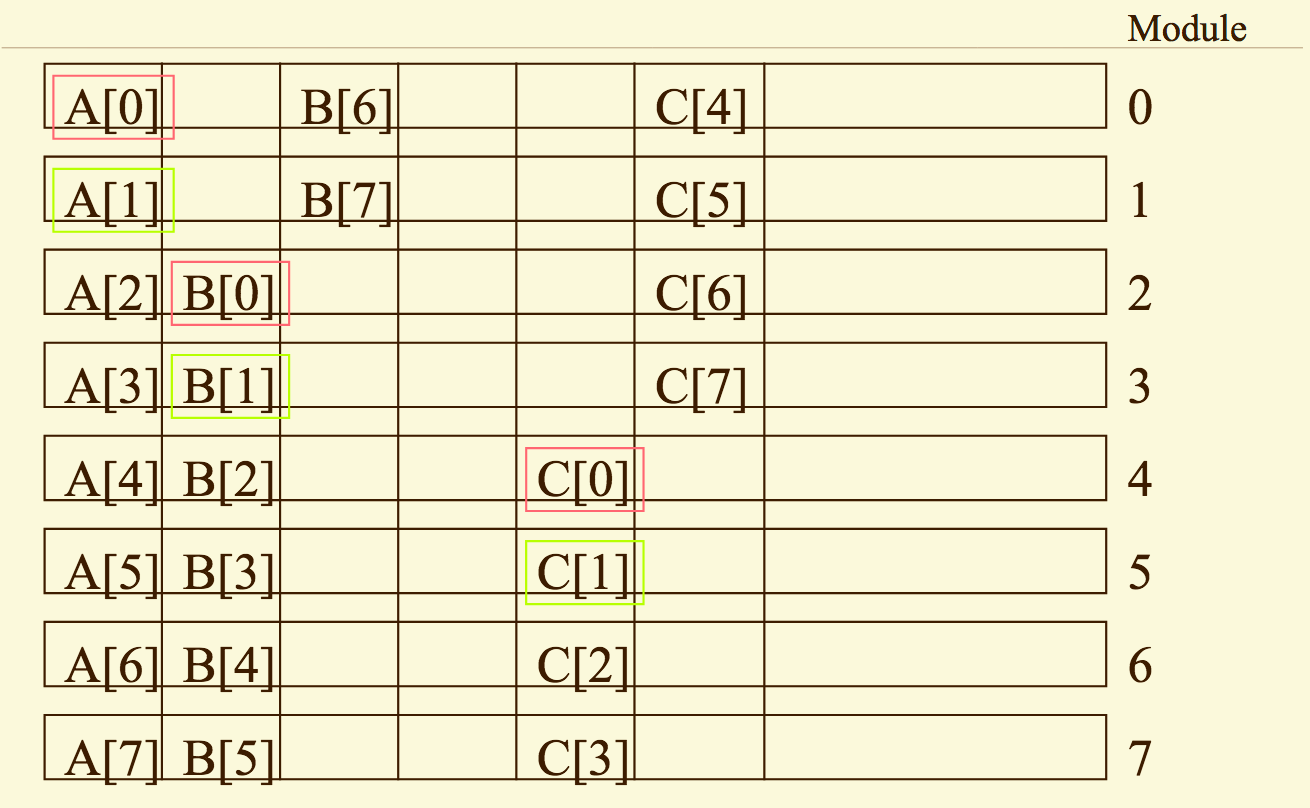
\includegraphics[width=0.7\linewidth]{figures/screenshot080}
\caption{Memory layout of an interleaved vector processing system.}
\label{fig:screenshot080}
\end{figure}

\begin{figure}
\centering
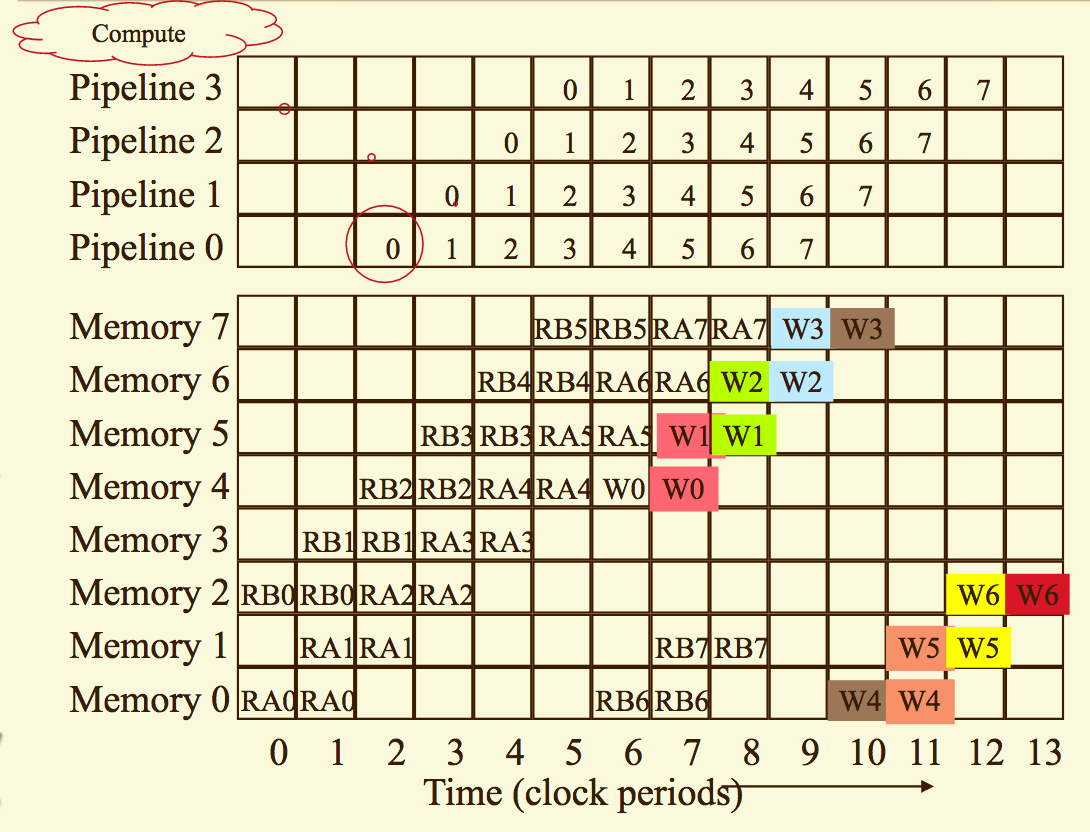
\includegraphics[width=0.7\linewidth]{figures/screenshot081}
\caption{Pipeline utilisation of an interleaved vector processing system.}
\label{fig:screenshot081}
\end{figure}

However, it is possible for memory contention to occur, as depicted in \autoref{fig:screenshot082}. To alleviate this, a delay path can be added to the pipelined adder (seen in \autoref{fig:screenshot083}) to mitigate this. The impact of doing this is seen in \autoref{fig:screenshot084}.

\begin{figure}
\centering
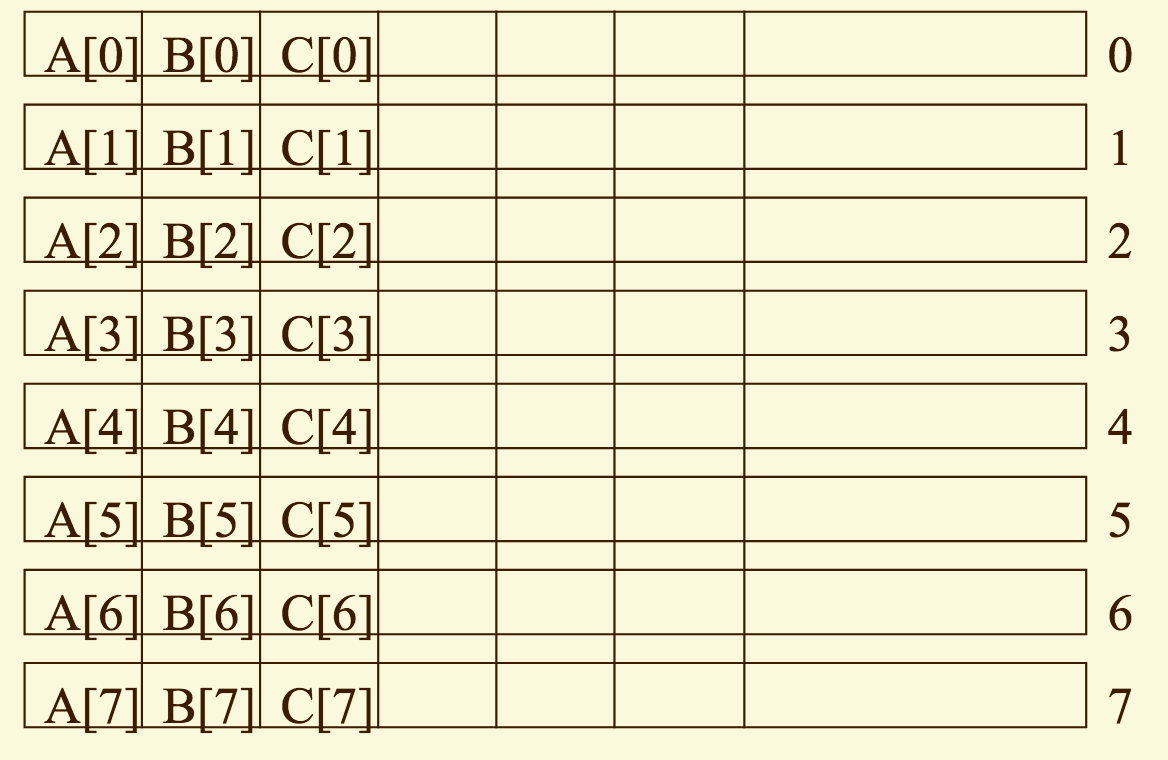
\includegraphics[width=0.7\linewidth]{figures/screenshot082}
\caption[Memory contention.]{Memory contention; these arrays are arranged in such a way that all accesses are on the same bank, dramatically slowing down processing.}
\label{fig:screenshot082}
\end{figure}

\begin{figure}
\centering
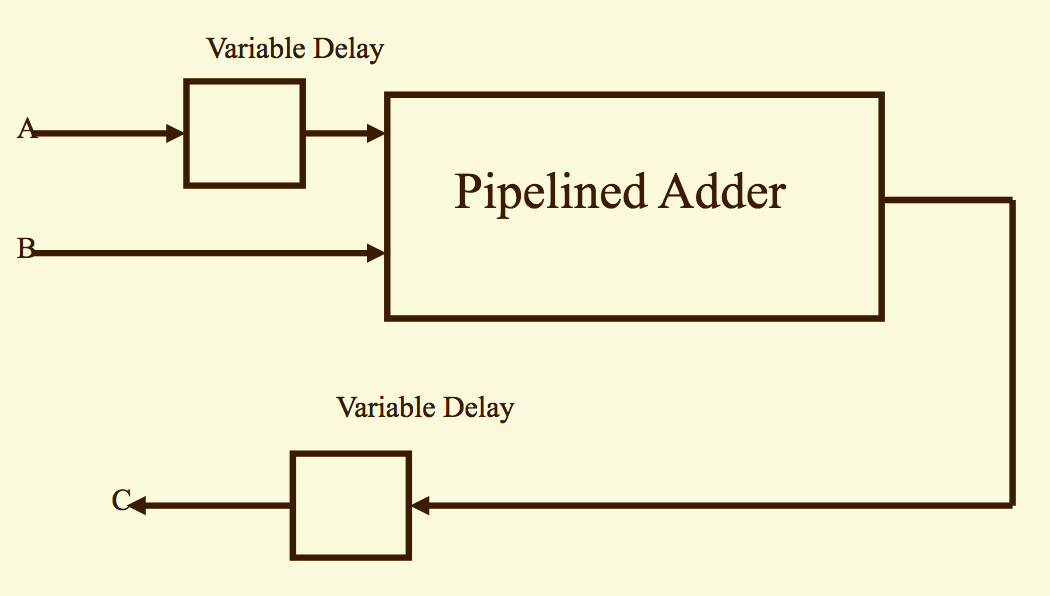
\includegraphics[width=0.7\linewidth]{figures/screenshot083}
\caption{Adding artificial delay paths to the pipelined adder.}
\label{fig:screenshot083}
\end{figure}

\begin{figure}
\centering
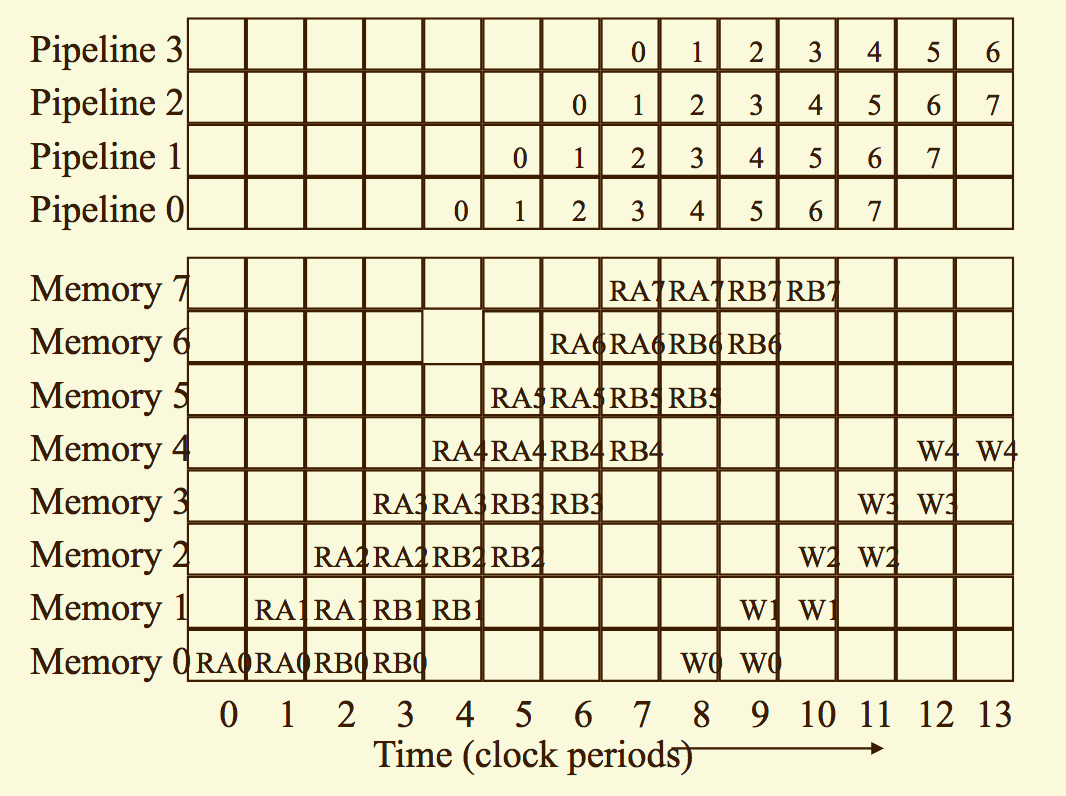
\includegraphics[width=0.7\linewidth]{figures/screenshot084}
\caption[Delay path pipelining.]{Pipelining after the delay path has been added. Note that the pipelines can run concurrently as the data they require has been made available by the delay.}
\label{fig:screenshot084}
\end{figure}

\section{CRAY-1}
The CRAY-1 has facilities for vector processing that work on a 64-word basis per vector. The compilers are vectorising, and can translate loops of serial operations into vector arithmetic. Additionally, the floating-point functional units can accept vector registers. This can be seen in \autoref{fig:screenshot085}.

\begin{figure}
\centering
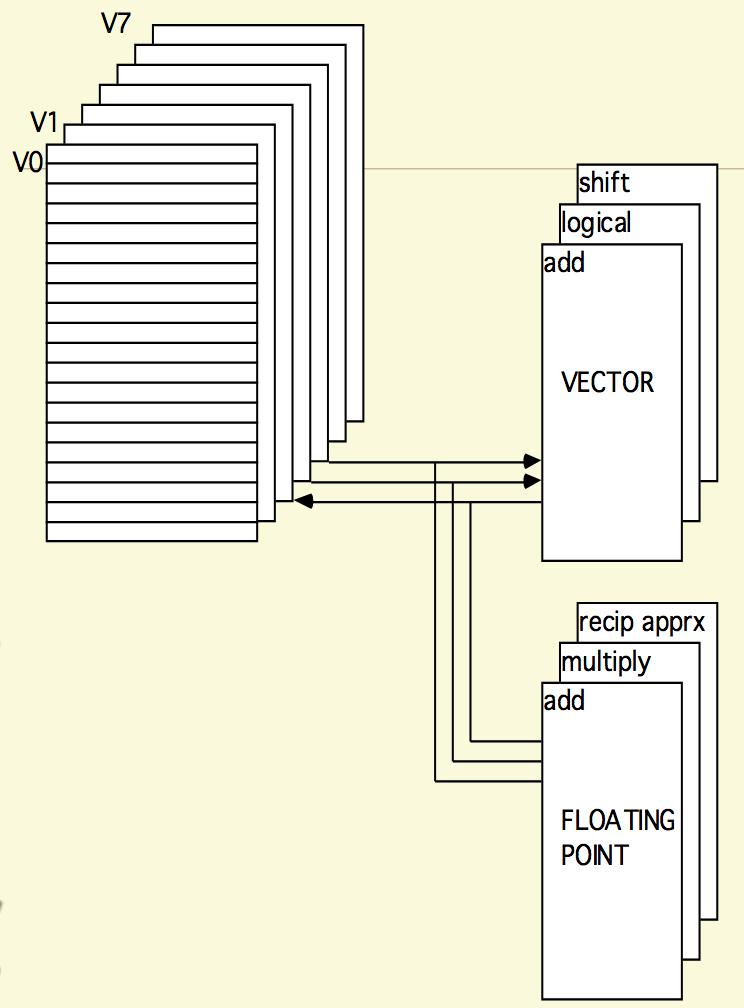
\includegraphics[width=0.7\linewidth]{figures/screenshot085}
\caption{CRAY-1 architecture.}
\label{fig:screenshot085}
\end{figure}

The CRAY-1 was capable of achieving even faster vector operations by using chaining. The result vector was not only sent to the destination vector register, but also directly to another functional unit. Data could be made to chain from one functional unit to another, potentially without any intermediate storage.

Vector instructions may be issued at the rate of one instruction per clock period; if there is no contention, they will generally be issued at this rate. The first result will appear after some delay, and then each word of the vector will arrive at the rate of one word per clock period. Vectors longer than 64 words are broken into 64 word chunks.

\section{Stride}
\label{sec:stride}
Most interleaving schemes take the bottom bits of the address to select the memory bank to use. This is excellent for sequential address patterns of a stride of 1 (that is, each access is one address apart), and acceptable for random access.

However, when the stride is $n$, where $n$ is a multiple of the number of memory banks (that is, each access is $n$ addresses apart), performance can be extremely poor. This is due to each access using the same memory bank; this effectively cripples any vectorisation capability, resulting in serialisation and thus a dramatic performance drop.

There has been significant research into mitigating the performance impact of $n \propto m$-stride, where $m$ is the number of memory banks. The two primary approaches are to arrange the data to match the stride (software), or to make the hardware insensitive to stride.

\subsection{Software}
Consider a 8x8 matrix; it can be placed in memory in either row or column order. If the program only needs to access the matrix in either row or column order, the order of the matrix can be chosen to guarantee conflict-free access.

Additionally, the matrix can be skewed so that each row starts in a different memory bank. This allows access by row or column order without memory contention. However, the software will need to ensure it accesses the matrix correctly.

\subsection{Hardware}
The hardware can use another function for determining which memory bank to use. This function can be optimised to provide stride-free access for many different strides. Additionally, there are schemes that give optimal packing and do not waste any space.

\subsection{Other}
However, row and column access are not necessarily the only methods of access. Other common modes of access are matrix diagonals and square subarrays of matrices.

The stride to access a diagonal element from the current element is equal to the column stride + 1. However, if $m$, the number of memory banks, is equal to a power of $2$, both column stride and column stride + 1 cannot both be efficient to access; this follows from the fact that both column stride and column stride + 1 cannot be relatively prime to $m$.

\section{Vector Algorithms}
\subsection{Gaussian Elimination}
Consider the solution of the linear equations given by $Ax = b$, where $A$ is a $N \times N$ matrix and $x$, $b$ are $N \times 1$ column vectors.

Gaussian elimination is an efficient algorithm for producing upper and lower diagonal matrices $L$ and $U$ such that $A = LU$. \footnote{Well \textit{actually}, this is LU decomposition.} Given $L$ and $U$, it is possible to write $Ly = b$ and $Ux = y$; this can then be used to solve for $x$ using backsubstitution.

This can be implemented as a vectorised algorithm \footnote{Nope, sorry, didn't want to rewrite this one as pseudocode either.}:
\begin{lstlisting}
for i := 1 to N do begin 
	imax := index of Max(abs(A[i..N,i])); 
	Swap(A[i,i..N],A[imax,i..N]); 
	if A[i,i] = 0 then Singular Matrix; 
	A[I+1..N,i] := A[I+1..N,i]/A[i,j]; 
	for k := i+1 to N do 
		A[k,i+1..N] := A[k,i+1..N] - A[k,i]*A[i,i+1..N]; 
end; 
\end{lstlisting}
The breakdown of $A$ can be seen in \autoref{fig:screenshot086}.

\begin{figure}
\centering
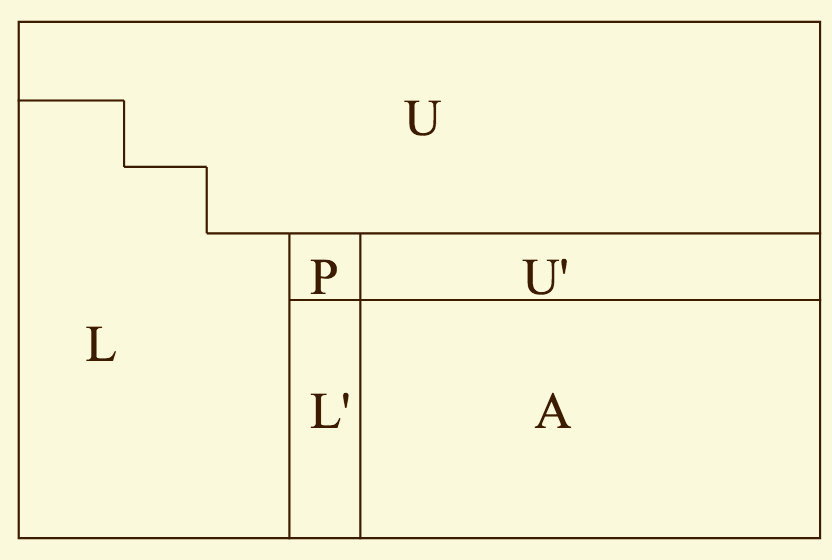
\includegraphics[width=0.7\linewidth]{figures/screenshot086}
\caption{Vectorised Gaussian elimination \footnotemark breakdown.}
\label{fig:screenshot086}
\end{figure}
\footnotetext{Yep, still LU decomposition}

The algorithm as expressed accesses both rows and columns. The majority of the vector operations have either two vector operands, or a scalar and a vector operand, and they produce a vector result. The \texttt{Max} operation on a vector returns the index of the maximum element, not the value of the maximum element. The length of the vector items accessed decreases by 1 for each successive iteration. 

It is worth noting that row and column access should be equally efficient (see \autoref{sec:stride}). Additionally, the vector pipeline should be able to handle a scalar on an input, and the \texttt{Min}, \texttt{Max} and \texttt{Sum} operators should accept one or more vectors and return a scalar. Finally, vectors may start large, but will get smaller. This may affect code generation due to the cost of initialising the vector units.

\subsection{Sparse Matrices}
In many engineering computations, there may be very large matrices. These are often sparely occupied, with many zero elements; this class of matrices are called \textit{sparse matrices}. Storing sparse matrices traditionally would occupy far too much memory, and be very slow to process.

Many software packages solve this problem by using a software data representation that \textit{does not} store elements with a zero value. They typically provide at least random and row/column sequential access to the sparse matrices.

Matrix multiplication will then consist of adjusting the pointers to the real data and multiplying elements if they share the same index values. In future, hardware may implement a matrix data representation suitable for sparse matrices.

\section{Random Figures}
These figures were at the end of the slides.

\begin{figure}
\centering
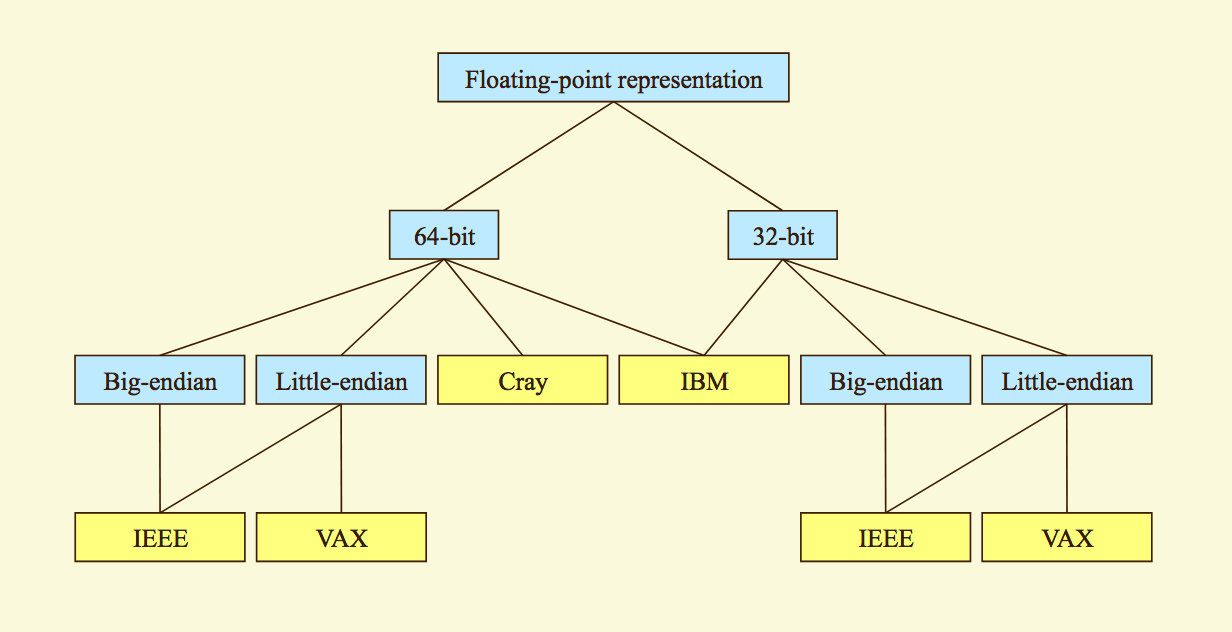
\includegraphics[width=0.5\linewidth]{figures/screenshot087}
\caption{The design space for floating-point precision.}
\label{fig:screenshot087}
\end{figure}

\begin{figure}
\centering
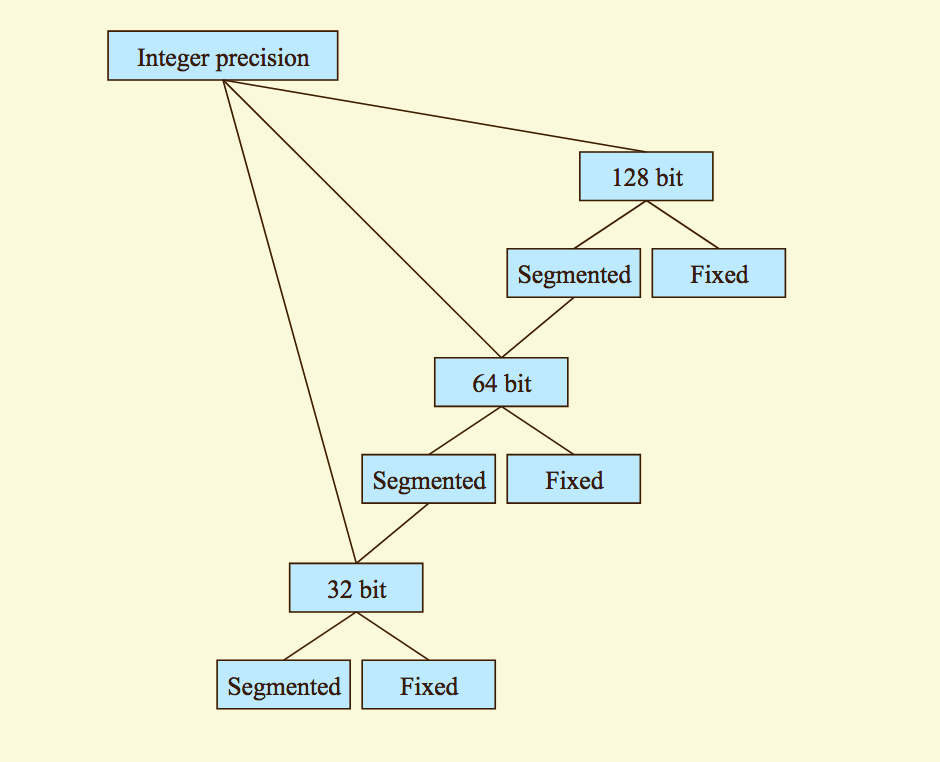
\includegraphics[width=0.5\linewidth]{figures/screenshot088}
\caption{The design space for integer precision.}
\label{fig:screenshot088}
\end{figure}

\begin{figure}
\centering
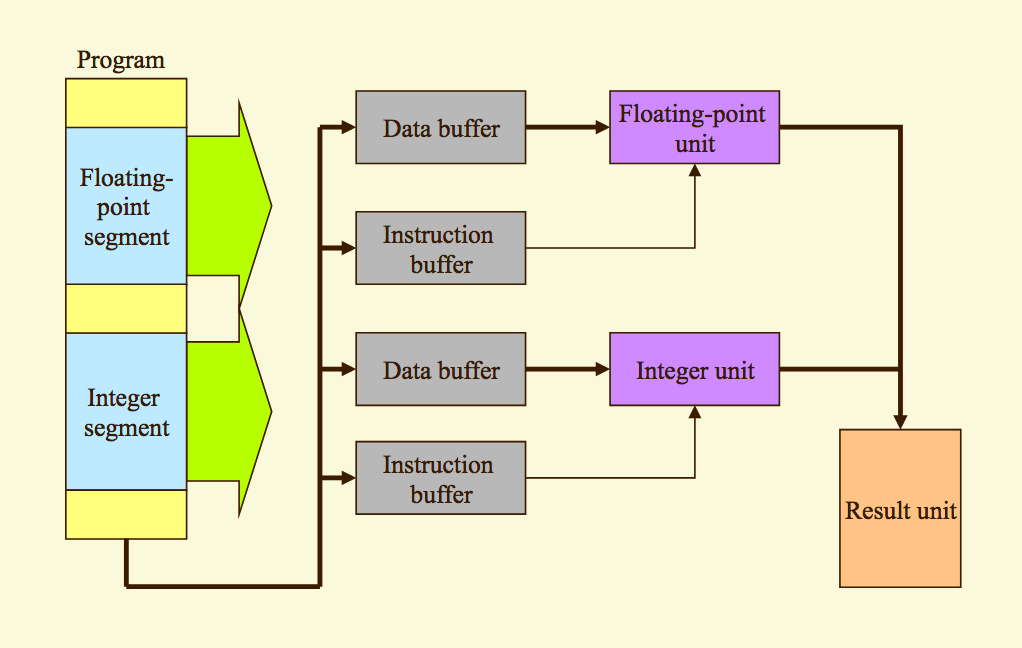
\includegraphics[width=0.5\linewidth]{figures/screenshot089}
\caption{Parallel computation of floating-point and integer results.}
\label{fig:screenshot089}
\end{figure}

\begin{figure}
\centering
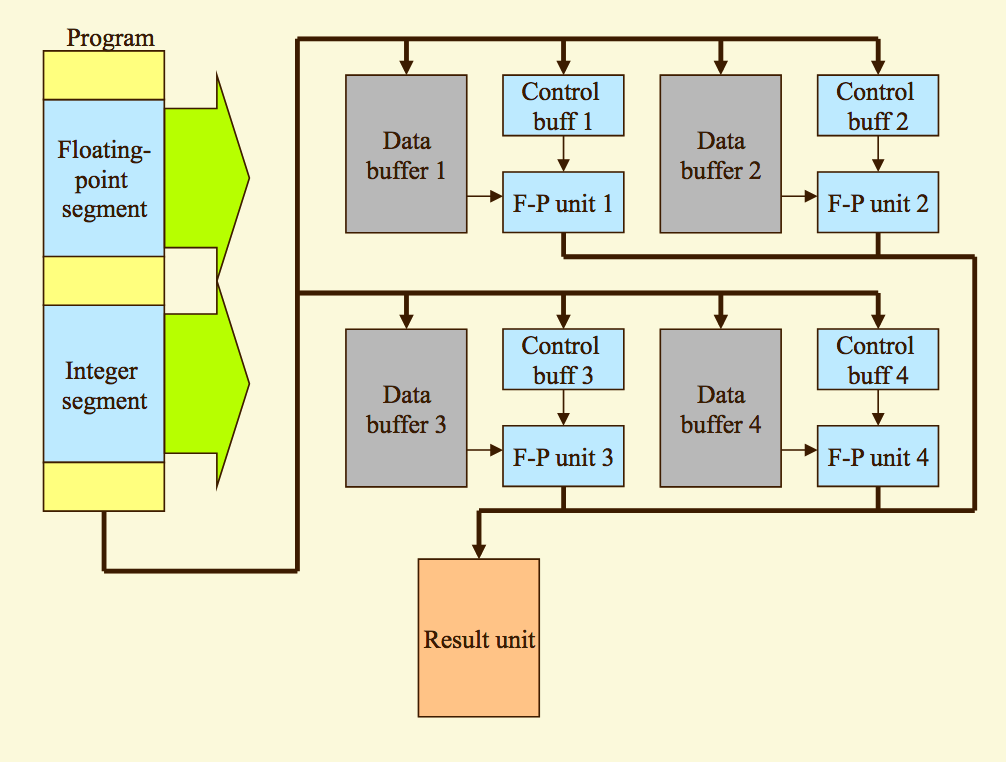
\includegraphics[width=0.5\linewidth]{figures/screenshot090}
\caption{Mixed function and data parallelism.}
\label{fig:screenshot090}
\end{figure}

\begin{figure}
\centering
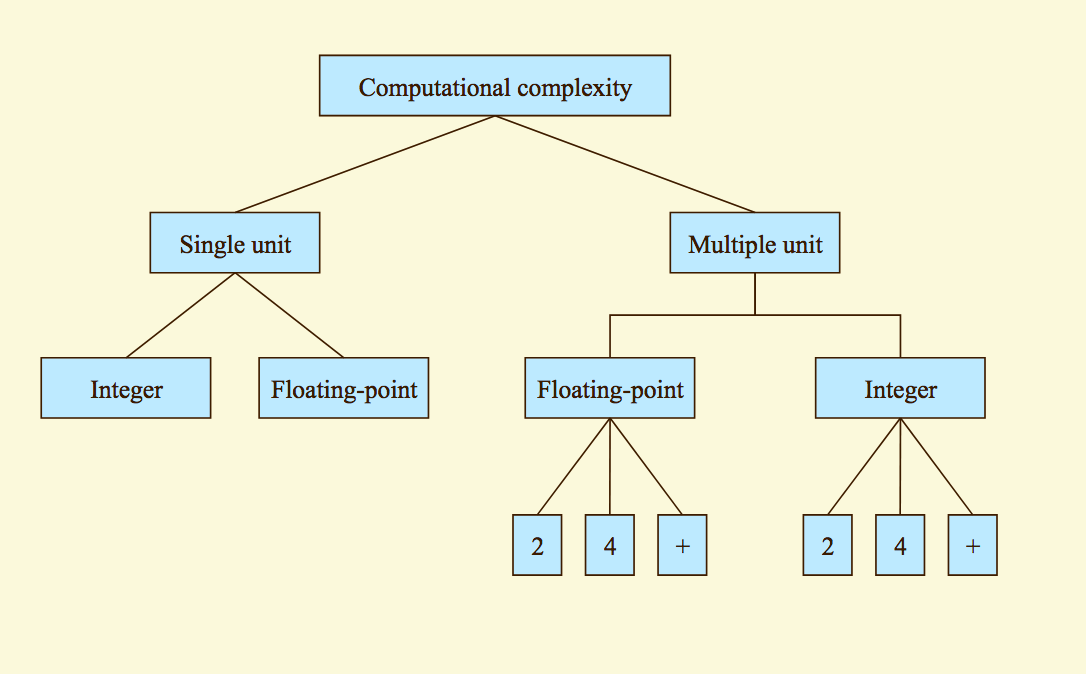
\includegraphics[width=0.5\linewidth]{figures/screenshot091}
\caption{The design space for parallel computational functionality.}
\label{fig:screenshot091}
\end{figure}

\begin{figure}
\centering
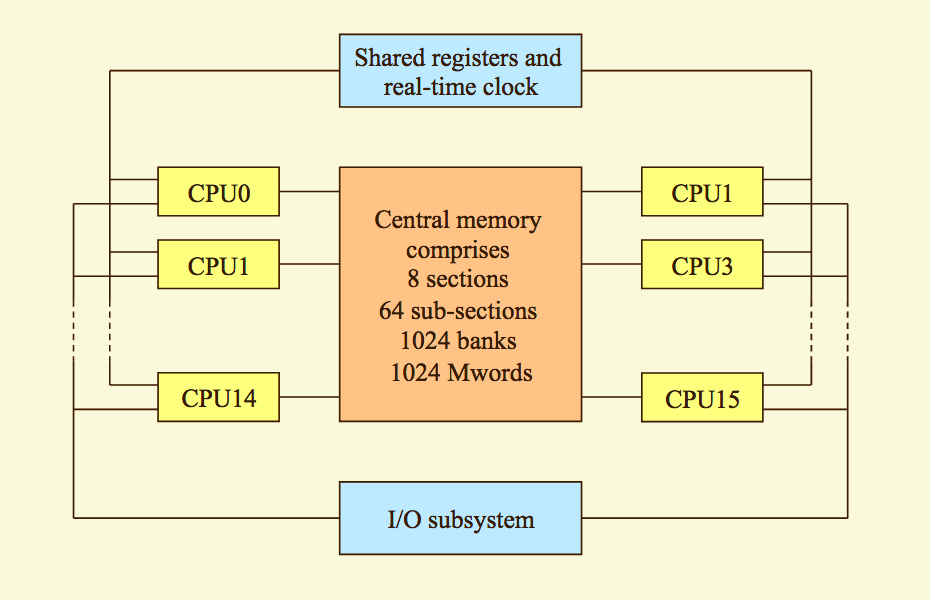
\includegraphics[width=0.5\linewidth]{figures/screenshot092}
\caption{Communication between CPUs and memory.}
\label{fig:screenshot092}
\end{figure}

\begin{figure}
\centering
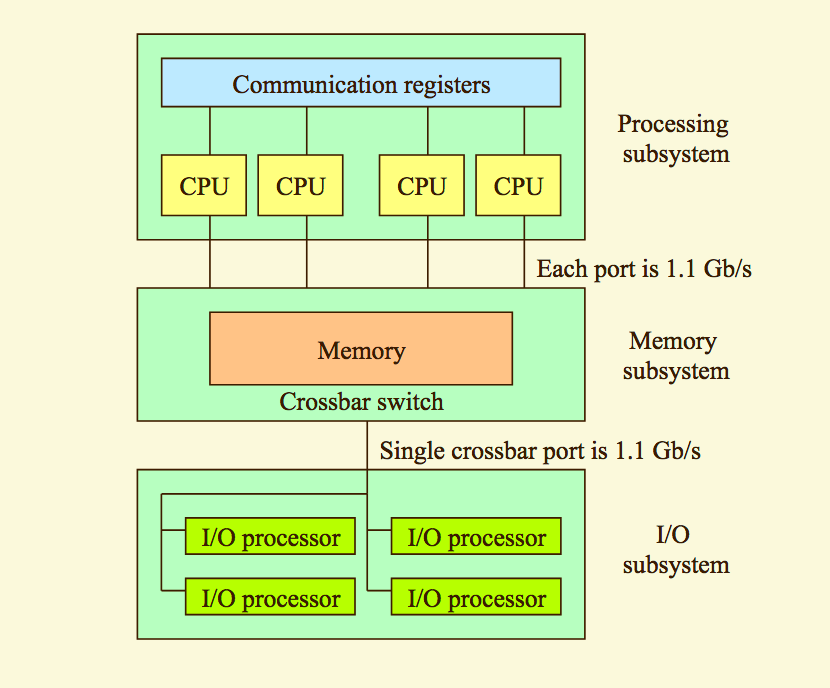
\includegraphics[width=0.5\linewidth]{figures/screenshot093}
\caption{The overall architecture of the Convex C4/XA system.}
\label{fig:screenshot093}
\end{figure}

\begin{figure}
\centering
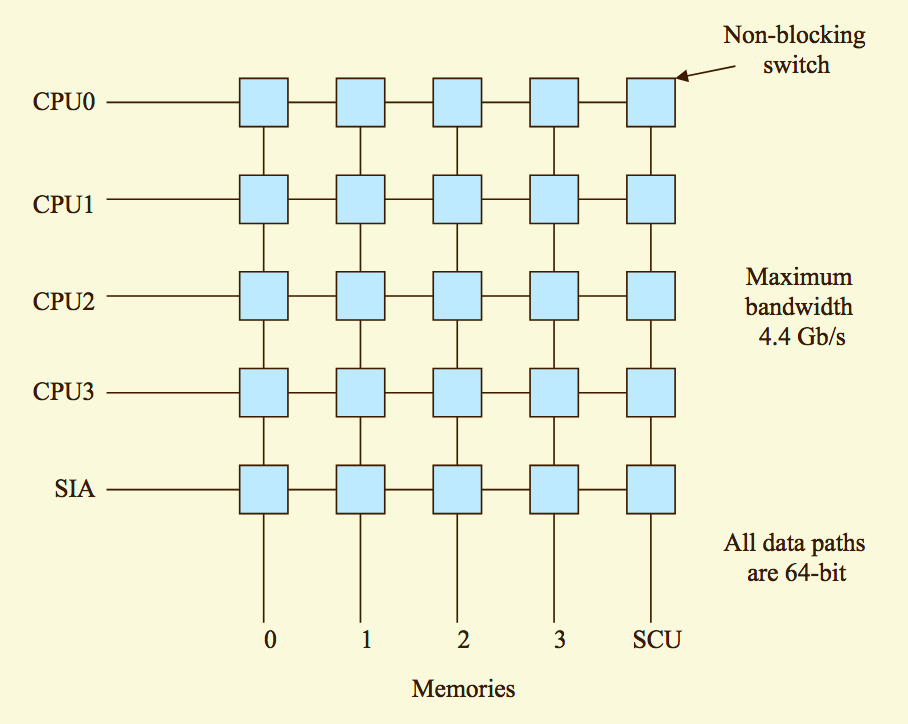
\includegraphics[width=0.5\linewidth]{figures/screenshot094}
\caption{The configuration of the crossbar switch.}
\label{fig:screenshot094}
\end{figure}

\begin{figure}
\centering
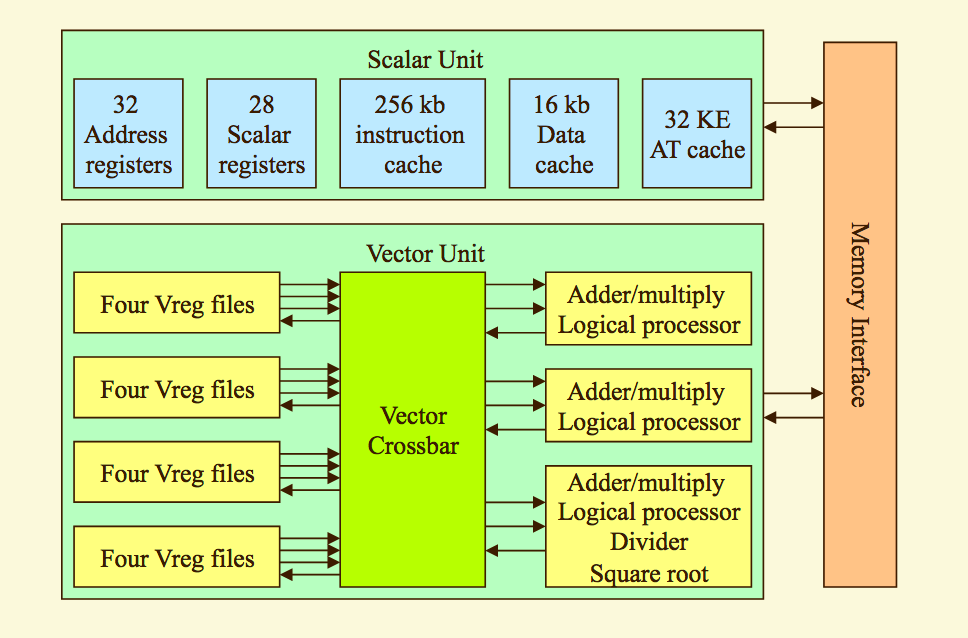
\includegraphics[width=0.5\linewidth]{figures/screenshot095}
\caption[The processor configuration.]{The processor configuration. (Some processor, anyway.)}
\label{fig:screenshot095}
\end{figure}

\pagebreak

Boy, that was a lot of figures. Wish I knew what they were for!
